\section{Verwitterung}
\begin{myExBox}[title=Verwitterung]
\textbf{Prozesse} der Lockerung, Aufbereitung und Zerstörung von Gesteinen sowie Mineralien an oder nahe der Erdoberfläche durch die Einwirkung \textbf{physikalischer} (mechanischer), \textbf{chemischer} oder \textbf{biogener} Einflüsse. Die Stärke der Verwitterung hängt ab vom Klima, den Eigenschaften des Gesteins sowie der Zeitdauer, während dem die Prozesse dauern.
\end{myExBox}

\notiz{8}
\newpage
\begin{myexercise}
Vervollständigen Sie folgende Tabelle beim Zuschauen des Films
\begin{table}[H]
\centering
\begin{tabular}{@{}l|p{5cm}||p{6cm}|p{2.5cm}@{}}
\toprule
\tiny Film \normalsize &\textbf{Verwitterungstyp} & \textbf{Beschreibung und Beispiele} & \textbf{Produkt} \\
\midrule\midrule
\tiny 2.1 &\textbf{Temperatur-Verwitterung\footnote{Wird auch Insolationsverwitterung genannt}} & & \\[50pt] \midrule
\tiny 2.2 &\textbf{Frost-Verwitterung}  & & \\[50pt] \midrule
\tiny 2.3 &\textbf{Salz-Verwitterung}  & & \\[50pt] \midrule
\tiny 2.4 &\textbf{Biologisch-physikalische Verwitterung}  & & \\[50pt]\midrule
-&\textbf{Druckentlastungs-Verwitterung}  & & \\[50pt]\bottomrule
\end{tabular}
\caption{Physikalische Verwitterung: Typen und Prozesse}
\end{table}
\begin{myanswer}
\begin{table}[H]
\centering
\begin{tabular}{@{}l|p{4cm}||p{6cm}|p{2.5cm}@{}}
\toprule
\tiny Film \normalsize &\textbf{Verwitterungstyp} & \textbf{Beschreibung und Beispiele} & \textbf{Produkt} \\
\midrule\midrule
\tiny 2.1 & \textbf{Temperatur-Verwitterung} & Temperaturschwankungen durch Sonneneinstrahlung: Erwärmung (Ausdehnung) am Tag, Abkühlung (Schrumpfung) in der Nacht erzeugen Spannungen. & Körnig-eckiger Gesteinsschutt \\\midrule
\tiny 2.2 & \textbf{Frost-Verwitterung} & Volumenvergrösserung von gefrierendem Wasser (um 9 \%) erzeugt Druck. & Blöcke \\\midrule
\tiny 2.3 & \textbf{Salz-Verwitterung} & Verdunstung von Wasser, Kristallisation der gelösten Salze. Ausdehnung durch Kristallisationsdruck führt zu Sprengung. & Rundliche Hohlräume \\\midrule
\tiny 2.4 & \textbf{Biologisch-physikalische\newline Verwitterung} & Sprengung durch Pflanzenwurzeln. & Blöcke \\\midrule
\tiny - & \textbf{Druckentlastungs-Verwitterung} & Abtragung von überlagerndem Gestein reduziert den Druck, wodurch sich das Gestein ausdehnt und in Schalen ablöst. & Schalenförmige Abplatzungen \\\bottomrule

\end{tabular}
\caption{Physikalische Verwitterung: Typen und Prozesse}
\end{table}
\end{myanswer}
\end{myexercise}
\newpage
\begin{myexercise}
Vervollständigen Sie folgende Tabelle während dem Zuschauen des Films
\begin{table}[H]
\centering
\begin{tabular}{@{}l|p{3cm}||p{6cm}|p{3cm}@{}}
\toprule
\tiny Film &\textbf{Verwitterungstyp} & \textbf{Beschreibung und Beispiele} & \textbf{Produkt} \\
\midrule\midrule
\tiny 3.1 & \textbf{Hydratations-Verwitterung} & &  \\[50pt] \midrule
\tiny 3.2, 3.3 & \textbf{Lösungs-Verwitterung \newline (Hydrolyse)} & & \\[50pt] \midrule
\tiny - &\textbf{Oxidations-Verwitterung} & & \\[50pt] \bottomrule

%\tiny - & \textbf{Biologisch-chemische Verwitterung} & & \\[50pt] \bottomrule
\end{tabular}
\caption{Chemische Verwitterung: Typen und Prozesse}
\end{table}
\begin{myanswer}
\begin{table}[H]
\centering
\begin{tabular}{@{}l|p{3cm}||p{6cm}|p{3cm}@{}}
\toprule
\small
\tiny Film &\textbf{Verwitterungstyp} & \textbf{Beschreibung und Beispiele} & \textbf{Produkt} \\
\midrule\midrule
\tiny 3.1 & \textbf{Hydratations-Verwitterung} & Volumenvergrösserung durch Anlagerung von Wassermolekülen im Kristallgitter von Mineralien. Kein Aufbrechen chemischer Verbindungen! & Zerfallene Mineralien \\\midrule
\tiny 3.2, 3.3 &\textbf{Lösungs-Verwitterung\newline (Hydrolyse)} & Lösen von Substanzen in Wasser, z.B. Steinsalz, Kalk, Gips. \newline Sonderformen: \textbf{Kohlensäureverwitterung} (siehe \cref{fig:ksverw}), \textbf{Rauchgasverwitterung}. Aufbrechen chemischer Bindungen. & Hartes Wasser \\\midrule
\tiny - &\textbf{Oxidations-Verwitterung} & Oxidation von z.B. Eisen mit Sauerstoff in Luft und/oder Wasser. & Rost \\\bottomrule

%\tiny - & \textbf{Biologisch-chemische Verwitterung} & Organische Säuren von Pflanzen lösen Mineralien auf. & Humus \\\bottomrule
\end{tabular}
\caption{Chemische Verwitterung: Typen und Prozesse}
\end{table}
\end{myanswer}
\end{myexercise}

\begin{figure}[H]
\centering
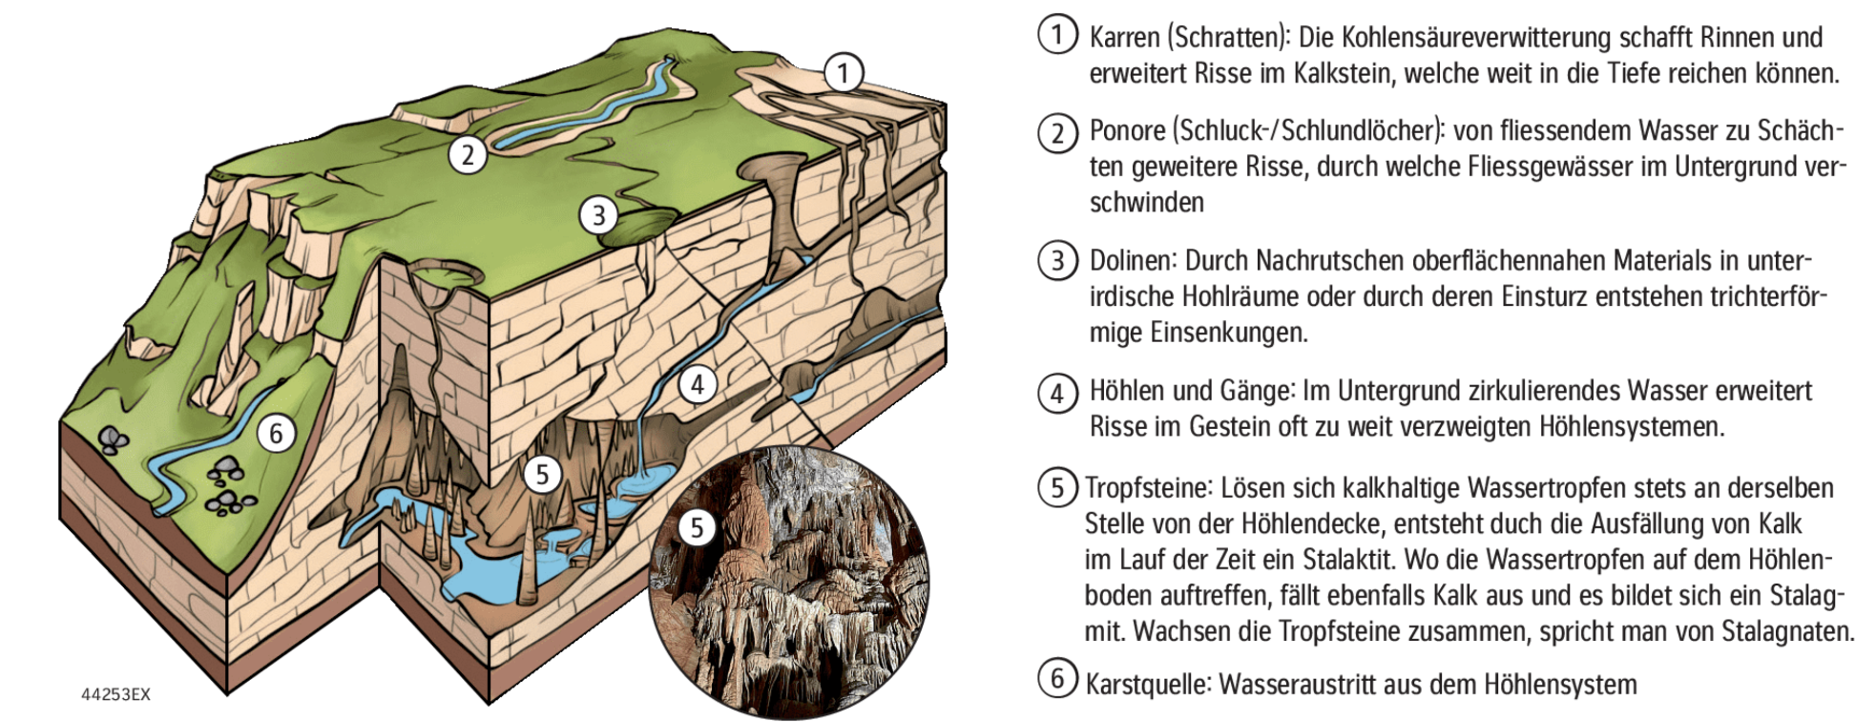
\includegraphics[width=.8\linewidth]{Geografie/Geomorphologie/Figures/Karst}
\caption{Ober- und unterirdische Karst-Formen als Resultat der Kohlensäureverwitterung \cite[132]{westermann}}
\label{fig:karst}
\end{figure}


\begin{figure}
\centering
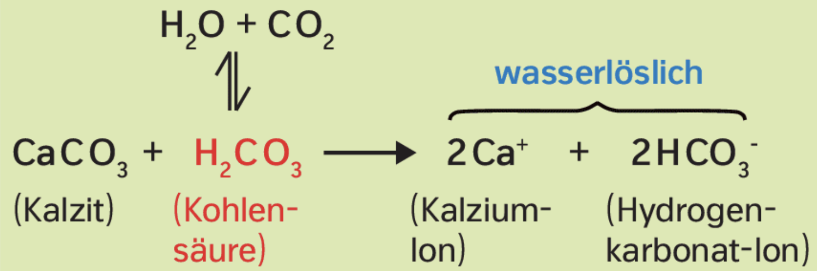
\includegraphics[width=0.5\linewidth]{Geografie/Geomorphologie/Figures/ksVerw}
\caption{Kohlensäure-Verwitterung: Chemische Verwitterung von Kalk (Kalzit) \cite{westermann}}
\label{fig:ksverw}
\end{figure}


\section{Erosion}
\begin{myExBox}[title=Abtragung]
Durch Wasser (Flusserosion), Wind (Winderosion oder Deflation) und Eis (Gletschererosion), jedoch auch unmittelbar durch die Schwerkraft (z.B. Bergsturz) wird das aufbereitete Gesteinsmaterial verlagert. Eine linienhafte Abtragung (z.B. Flüsse) wird als \textbf{Erosion}, eine eher flächenhafte hingegen als \textbf{Denudation} bezeichnet.
\end{myExBox}
\notiz{5}
\begin{myExBox}[title=Ablagerung]
Nach dem Transport durch Wasser, Wind und Eis werden die festen Stoffe an bestimmten Orten wieder abgesetzt oder ausgeschieden, was man allgemein als Ablagerung, Akkumulation oder Sedimentation bezeichnet. Dabei unterscheidet man zwischen klastischen (z.B. Sand), chemischen (z.B. Gips) und biogenen Sedimenten (z.B. Korallenriff)
\end{myExBox}
\notiz{5}

\begin{myexercise}[(Quelle: \cite{hep})]
Die Alpen heben sich seit circa 30 Millionen Jahren um durchschnittlich 0.5 bis 1 mm pro Jahr. Damit sollten die höchsten Berggipfel heute eigentlich 15'000 bis 30'000 m hoch sein.

\begin{enumerate}
\item Wieso erreichen die Alpen \enquote{nur} circa 4000 m Höhe?
\item Überprüfen Sie Ihre Hypothesen mit dem Kapitel 3.3 im Buch \enquote{Diercke Geografie}\cite{westermann} und diskutieren Sie zu zweit anhand des Fotos, welche Verwitterungsarten aus welchem Grund im Gebiet des Altels vorkommen beziehungsweise nicht vorkommen.
\end{enumerate}
\begin{figure}[H]
\centering
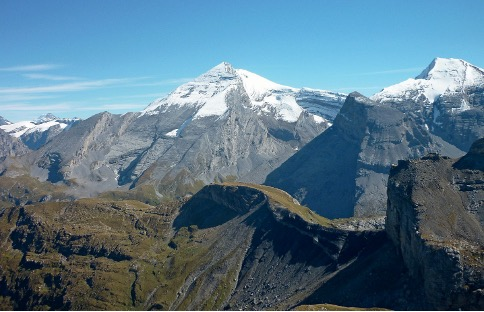
\includegraphics[width=0.7\linewidth]{Geografie/Geomorphologie/Figures/Altels}
\caption{Der Altels im Berner Oberland, 3629 m ü. M. (© Fritz Lauber).}
\label{fig:altels}
\end{figure}
\begin{myanswer}
Die Alpen sind heute nicht 30'000 m hoch: Die Alpen erreichen heute \enquote{nur} eine Höhe von circa 4000 m, weil in den letzten 30 Millionen Jahren neben der Hebung der Alpen auch die Verwitterung das feste Gestein aufgelockert, zerkleinert oder aufgelöst und so die Abtragung des Gesteinsmaterials durch Flüsse und Gletscher ermöglicht hat.

\textbf{Physikalische Verwitterung} im Gebiet des Altels
\begin{itemize}
\item Neben Temperaturverwitterung dominiert Frostsprengung, da im Hochgebirge die Oberflächentemperatur von Gestein täglich um bis zu 100 °C schwanken kann und dabei auch Wasser in feinen Gesteinsklüften immer wieder gefriert und wieder auftaut. Die abgesprengten Gesteinsblöcke unterhalb von Felsbändern deuten auf beide Verwitterungsarten hin.
\item Wurzelsprengung kommt nicht vor, da in dieser Höhenlage kaum Vegetation vorhanden ist.
\item Salzsprengung tritt kaum auf, da bei den Temperaturen in diesen Höhenlagen das Wasser in den Gesteinsklüften kaum verdunstet, was für die Auskristallisation und die Volumenvergrösserung der Salze notwendig wäre.
\end{itemize}
\textbf{Chemische Verwitterung} im Gebiet des Altels
\begin{itemize}
\item Kohlensäureverwitterung tritt auf, da das Gebiet des Altels vorwiegend aus Kalk (mesozoische Sedimente) besteht.
\item Hydratations-, Lösungs-, Rauchgas- und Oxidations-Verwitterung treten kaum auf, da die Temperaturen zu tief sind die Luft relativ rein ist.
\end{itemize}
\end{myanswer}
\end{myexercise}

\begin{myexercise}
Lösen Sie das Quiz auf folgender Adresse: \qrcode{https://cblum.ch/quiz-geomorphologie/}
\end{myexercise}

\begin{mychallenge}
(Aus \cite[133]{westermann}) In welchen Gegenden der Schweiz würden Sie folgende Verwitterungsarten am ehesten erwarten?
\begin{enumerate}
\item Druckentlastungsverwitterung
\item Kohlensäureverwitterung
\end{enumerate}
\begin{figure}[H]
\centering
% 
\includegraphics[width=\linewidth]{Geografie/Geomorphologie/Figures/Geol_Karte_Schweiz}
\caption{Geologische Karte der Schweiz}
\label{fig:geolkarteschweiz}
\end{figure}
\begin{myanswer}
\begin{enumerate}
\item \textbf{Druckentlastungsverwitterung}: Granit- und Gneis, also Aarmassiv, Gotthardmassiv, Nordtessin, Teile des Wallis
\item \textbf{Kohlensäureverwitterung}: Kalkstein, also Jura und nördliche Alpen
\end{enumerate}
\end{myanswer}
\end{mychallenge}